%\documentclass[compress]{beamer}
\documentclass[handout]{beamer}
%\documentclass{beamer}
\usepackage[T1]{fontenc}
\usepackage{pifont}
\usepackage{threeparttable}
\usepackage{subcaption}
\usepackage{tikz-qtree}
\usepackage{listings}
\usepackage[american]{babel}
\usepackage{csquotes}
\usepackage[style=apa, backend=biber]{biblatex}
\usepackage{tikz}
\usepackage{multicol}
\usepackage{booktabs}
\usepackage{graphicx}
\usepackage{neuralnetwork}
\usepackage{hyperref}
\usepackage{fancyvrb}

\usepackage{minted}
\definecolor{listingbg}{rgb}{0.87,0.93,1}
\setminted[python]{
breaklines,
linenos,
fontsize=\scriptsize,
frame=single,
xleftmargin=0pt}

\hypersetup{
    pdfborder={0 0 0},
    colorlinks=true,
}
\usetheme[block=fill,subsectionpage=progressbar,sectionpage=progressbar]{metropolis} 

\definecolor{Purple}{HTML}{911146}
\definecolor{Orange}{HTML}{CF4A30}

\setbeamercolor{alerted text}{fg=Orange}
\setbeamercolor{frametitle}{bg=Purple}

\setbeamercovered{still covered={\opaqueness<1->{5}},again covered={\opaqueness<1->{100}}}

\lstset{
    basicstyle=\scriptsize\ttfamily,
    columns=flexible,
    breaklines=true,
    numbers=left,
    %stepsize=1,
    numberstyle=\tiny,
    backgroundcolor=\color[rgb]{0.85,0.90,1}
}

\lstnewenvironment{lstlistingoutput}{\lstset{
        basicstyle=\footnotesize\ttfamily,
        columns=flexible,
        breaklines=true,
        numbers=left,
        %stepsize=1,
        numberstyle=\tiny,
        backgroundcolor=\color[rgb]{.7,.7,.7}}}{}


\lstnewenvironment{lstlistingoutputtiny}{\lstset{
        basicstyle=\tiny\ttfamily,
        columns=flexible,
        breaklines=true,
        numbers=left,
        %stepsize=1,
        numberstyle=\tiny,
        backgroundcolor=\color[rgb]{.7,.7,.7}}}{}

\renewcommand*{\bibfont}{\tiny}

\makeatletter
\setbeamertemplate{headline}{%
    \begin{beamercolorbox}[colsep=1.5pt]{upper separation line head}
    \end{beamercolorbox}
    \begin{beamercolorbox}{section in head/foot}
        \vskip2pt\insertnavigation{\paperwidth}\vskip2pt
    \end{beamercolorbox}%
    \begin{beamercolorbox}[colsep=1.5pt]{lower separation line head}
    \end{beamercolorbox}
}
\makeatother

\newcommand{\question}[1]{
    \begin{frame}[plain]
        \begin{columns}
            \column{.4\textwidth}
            \makebox[\columnwidth]{
                
\includegraphics[width=\columnwidth,height=\paperheight,keepaspectratio]{mannetje.png}}
            \column{.6\textwidth}
            \large
            \textcolor{orange}{\textbf{\emph{#1}}}
        \end{columns}
    \end{frame}}

\newcommand{\instruction}[1]{\emph{\textcolor{gray}{[#1]}}}


\addbibresource{resources/literature.bib}

\graphicspath{{resources/pictures/}}

\title[Computational Communication Science 2]{\textbf{Computational Communication Science 2} \\Week 2 - Lecture\\ \emph{Bottom-up Approaches to Text Analysis: From Preprocessing to Vectorization}}
\author[Anne Kroon]{Anne Kroon \\ \footnotesize{a.c.kroon@uva.nl, @annekroon}}
\date{April 7, 2025}
\institute[Digital Society Minor, University of Amsterdam]{Digital Society Minor, University of Amsterdam}

\begin{document}

\begin{frame}{}
	\titlepage
\end{frame}

\begin{frame}{Today’s Agenda}
	\begin{tiny}
		\tableofcontents
	\end{tiny}
\end{frame}

\section{Recap: What We Covered Last Week}

\begin{frame}{Review of Key Concepts}
	\begin{itemize}
		\item \textbf{Text Preprocessing:} Cleaning and preparing raw text for analysis.
		\item \textbf{Core Techniques:}
		\begin{itemize}
			\item Stopword removal
			\item Stemming and lemmatization
			\item Using built-in string methods for text cleaning
		\end{itemize}
		\item \textbf{Methodological Approaches:} Combining \emph{bottom-up} (data-driven) and \emph{top-down} (theory-driven) approaches.
	\end{itemize}
\end{frame}

\begin{frame}{Typical preprocessing steps}
	\begin{block}{Preprocessing steps}
		\begin{description}
			\item [\emph{tokenization}] How do we (best) split a sentence into tokens (terms, words)?
			\item [\emph{pruning}] How can we remove unneccessary words/ punctuation?
			\item [\emph{lemmatization and stemming}] How can we make sure that slight variations of the same word are not counted differently?
			\item [\emph{ngrams}] Neighbouring terms
		\end{description}
	\end{block}
\end{frame}


\begin{frame}[fragile]{Tokenization and Document-Term Matrix (DTM)}
\textbf{Tokenization:} Splitting text into words or subwords.
\begin{minted}[breaklines, fontsize=\scriptsize]{python}
from nltk.tokenize import TreebankWordTokenizer
tokens = [TreebankWordTokenizer().tokenize(d) for d in docs]
\end{minted}
\end{frame}

\begin{frame}[fragile]{Understanding N-grams}
	\begin{itemize}
		\item An n-gram is a sequence of \(n\) words treated as a single feature.
		\item Examples:
		\begin{itemize}
			\item Unigrams (1-word units): “science”
			\item Bigrams (2-word units): “data science”
			\item Trigrams (3-word units): “machine learning model”
		\end{itemize}
		\item \textbf{Why use n-grams?} Captures context and word relationships beyond single words.
	\end{itemize}
\end{frame}

\begin{frame}[fragile]{Stemming and Lemmatization}
	\begin{itemize}
		\item \textbf{Stemming:} Reduces words to their base form (e.g., “running” → “run”).
		\item \textbf{Lemmatization:} Maps words to their dictionary form (e.g., “better” → “good”).
		\item Stemming is fast but can produce non-standard words; lemmatization is more accurate but computationally expensive.
	\end{itemize}
\begin{minted}[breaklines, fontsize=\scriptsize]{python}
from nltk.stem import PorterStemmer
stemmer = PorterStemmer()
tokens_stemmed = [stemmer.stem(word) for word in tokens]
\end{minted}
\end{frame}


\begin{frame}{Exercise time: Word cloud}
    \textbf{Let's put this into practice!}  
    \begin{itemize}
        \item Follow the instructions in the exercise material.
        \item You will create a word cloud from text data.
        \item Apply preprocessing techniques such as tokenization, stopword removal, and normalization.
    \end{itemize}
    \vspace{1cm}

\textbf{Exercise Link:}  
    \href{https://github.com/uva-cw-ccs2/2425s2/blob/main/week02/exercise-lecture/word-cloud-exercise.md}{GitHub: Word cloud exercise}  
    \vspace{1cm}
    
    �� \textbf{Time:} 5 minutes  

    \vspace{0.5cm}    
 \textit{Tip: Think about how different preprocessing choices impact the resulting word cloud!}
\end{frame}


\section{Building text representations: vectorizers}

\subsection{General idea}

\begin{frame}[fragile]{A text as a collections of word}
	
	Let us represent a string 
\begin{minted}[%
	breaklines,
	linenos,
	fontsize=\scriptsize,
	frame=single,
	xleftmargin=0pt,]
	{python}
t = "This this is is is a test test test"
# like this:
print(Counter(t.split()))
\end{minted}
\begin{minted}[%
	breaklines,
	fontsize=\scriptsize,]
	{python}
Counter({'is': 3, 'test': 3, 'This': 1, 'this': 1, 'a': 1})
\end{minted}
	
	\pause 
	Compared to the original string, this representation
	\begin{itemize}
		\item is less repetitive
		\item preserves word frequencies
		\item but does \emph{not} preserve word order
		\item can be interpreted as a vector to calculate with (!!!)
	\end{itemize}
	
	\tiny{\emph{Of course, still a lot of stuff to fine-tune\ldots}  (for example, This/this)}
\end{frame}


\begin{frame}{From vector to matrix}
	If we do this for multiple texts, we can arrange the vectors in a table.
	
	t1 = "This this is is is a test test test" \newline
	t2 = "This is an example"
	
	\begin{tabular}{| c|c|c|c|c|c|c|c|}
		\hline
		& a & an & example & is & this & This & test \\
		\hline
		\emph{t1} & 1 & 0 & 0 & 3 & 1 & 1 & 3 \\
		\emph{t2} &0 & 1 & 1 & 1 & 0 & 1 & 0 \\
		\hline
	\end{tabular}
\end{frame}

\question{What can you do with such a matrix? Why would you want to represent a collection of texts in such a way?}

\begin{frame}{What is a vectorizer}
	\begin{itemize}[<+->]
		\item Transforms a list of texts into a sparse (!) matrix (of word frequencies)
		\item Vectorizer needs to be ``fitted'' to the training data (learn which words (features) exist in the dataset and assign them to columns in the matrix)
		\item Vectorizer can then be re-used to transform other datasets 
	\end{itemize}
\end{frame}


\begin{frame}{The cell entries: raw counts versus tf$\cdot$idf scores}
	\begin{itemize}
		\item In the example, we entered simple counts (the ``term frequency'')
	\end{itemize}
\end{frame}

\question{But are all terms equally important?}


\begin{frame}{The cell entries: raw counts versus tf$\cdot$idf scores}
	\begin{itemize}
		\item In the example, we entered simple counts (the ``term frequency'')
		\item But does a word that occurs in almost all documents contain much information?
		\item And isn't the presence of a word that occurs in very few documents a pretty strong hint?
		\item<2-> \textbf{Solution: Weigh by \emph{the number of documents in which the term occurs at least once) (the ``document frequency'')}} 
	\end{itemize}
	\onslide<3->{
		$\Rightarrow$ we multiply the ``term frequency'' (tf) by the inverse document frequency (idf)
		
		\tiny{(usually with some additional logarithmic transformation and normalization applied, see \url{https://scikit-learn.org/stable/modules/generated/sklearn.feature_extraction.text.TfidfTransformer.html})}
	}
\end{frame}

\begin{frame}{TF-IDF: Weighted Importance of Words}
\begin{itemize}
    \item Some words are more informative than others.
    \item \textbf{TF-IDF} adjusts for term frequency and rarity across documents.
\end{itemize}

\[
\text{tf-idf} = \text{tf}_{i,j} \times \log \left(\frac{N}{\text{df}_i}\right)
\]

\begin{itemize}
    \item \( \text{tf}_{i,j} \) = term frequency of term \( i \) in document \( j \)
    \item \( \text{df}_i \) = number of documents containing the term \( i \)
    \item \( N \) = total number of documents in the corpus
\end{itemize}

\vspace{0.5cm}
\textbf{Explanation:}
\begin{itemize}
    \item \textbf{Term Frequency (TF)}: Measures how often a term appears in a document. More frequent terms in a document receive a higher TF score.
    \item \textbf{Inverse Document Frequency (IDF)}: Downscales terms that appear in many documents and boosts those that are rare but important.
    \item If a term appears frequently in a document but is rare in the overall corpus, it gets a high TF-IDF score, indicating its significance.
    \item Common words (e.g., "the", "and") appear in many documents, leading to a low IDF score and reducing their weight.
\end{itemize}

\textbf{Use Case:}  
TF-IDF is widely used in information retrieval, search engines, and text mining to identify the most relevant words that uniquely characterize a document.
\end{frame}


\begin{frame}{Is tf$\cdot$idf always better?}
	It depends.
	
	\begin{itemize}
		\item Ultimately, it's an empirical question which works better ($\rightarrow$ machine learning)
		\item In many scenarios,  ``discounting'' too frequent words and ``boosting'' rare words makes a lot of sense (most frequent words in a text can be highly un-informative)
		\item Beauty of raw tf counts, though: interpretability + describes document in itself, not in relation to other documents
	\end{itemize}
\end{frame}


\begin{frame}{Different vectorizers}
	\begin{enumerate}[<+->]
		\item CountVectorizer (=simple word counts)
		\item TfidfVectorizer (word counts (``term frequency'') weighted by number of documents in which the word occurs at all (``inverse document frequency''))
	\end{enumerate}
\end{frame}

\begin{frame}{Internal representations}
	\begin{block}{Sparse vs dense matrices}
		\begin{itemize}
			\item $\rightarrow$ tens of thousands of columns (terms), and one row per document
			\item Filling all cells is inefficient \emph{and} can make the matrix too large to fit in memory (!!!)
			\item Solution: store only non-zero values with their coordinates! (sparse matrix)
			\item dense matrix (or dataframes) not advisable, only for toy examples
		\end{itemize}
	\end{block}
\end{frame}


{\setbeamercolor{background canvas}{bg=black}
	\begin{frame}
		\makebox[\linewidth]{
			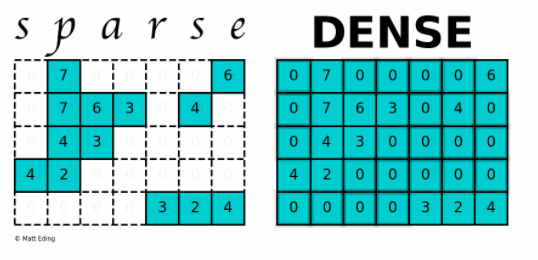
\includegraphics[width=\paperwidth,height=\paperheight,keepaspectratio]{sparse_dense.png}}
		\url{https://matteding.github.io/2019/04/25/sparse-matrices/}
	\end{frame}
}


\begin{frame}[fragile]
We learned in week 1 how to tokenize with a list comprehension (and that's often a good idea!). 

\begin{minted}[%
	breaklines,
	fontsize=\scriptsize,]
	{python}
from nltk.tokenize import TreebankWordTokenizer
tokens = [TreebankWordTokenizer().tokenize(d) for d in docs]
\end{minted}

But what if we want to \emph{directly} get a DTM instead of lists of tokens?
\end{frame}

\begin{frame}[fragile]{OK, good enough, perfect?}
	\begin{block}{scikit-learn's CountVectorizer (default settings)}
		\begin{itemize}
			\item applies lowercasing
			\item deals with punctuation etc. itself
			\item minimum word length $>1$
			\item more technically, tokenizes using this regular expression: \texttt{r"(?u)\textbackslash b\textbackslash w\textbackslash w+\textbackslash b"} \footnote{?u = support unicode, \textbackslash b = word boundary}
		\end{itemize}
	\end{block}
\begin{minted}[%
	breaklines,
	linenos,
	fontsize=\scriptsize,
	frame=single,
	xleftmargin=0pt,]
	{python}
from sklearn.feature_extraction.text import CountVectorizer
cv = CountVectorizer()
dtm_sparse = cv.fit_transform(docs)
\end{minted}
\end{frame}


\begin{frame}{OK, good enough, perfect?}
	\begin{block}{CountVectorizer supports more}
		\begin{itemize}
			\item stopword removal
			\item custom regular expression
			\item or even using an external tokenizer
			\item ngrams instead of unigrams
		\end{itemize}
	\end{block}
	\tiny{see \url{https://scikit-learn.org/stable/modules/generated/sklearn.feature\_extraction.text.CountVectorizer.html}}
	
	\pause
	\begin{alertblock}{Best of both worlds}
		\textbf{Use the Count vectorizer with a NLTK-based external tokenizer! (see book)}
	\end{alertblock}
\href{https://github.com/uva-cw-ccs2/2425s2/blob/main/week02/exercise-lecture/Understanding_vectorizers.ipynb}{THis notebook might help to better your understanding of vectorizers!}  
\end{frame}


\subsection{Pruning}

\begin{frame}{General idea}
	\begin{itemize}
		\item Idea behind both stopword removal and tf$\cdot$idf: too frequent words are uninformative
		\item<2-> (possible) downside stopword removal: a priori list, does not take empirical frequencies in dataset into account
		\item<3-> (possible) downside tf$\cdot$idf: does not reduce number of features
	\end{itemize}
	
	\onslide<4->{Pruning: remove all features (tokens) that occur in less than X or more than X of the documents}
\end{frame}

\begin{frame}[fragile, plain]
	CountVectorizer, only stopword removal
\begin{minted}[%
	breaklines,
	linenos,
	fontsize=\tiny,
	frame=single,
	xleftmargin=0pt,]
	{python}
from sklearn.feature_extraction.text import CountVectorizer, TfidfVectorizer
myvectorizer = CountVectorizer(stop_words=mystopwords)
\end{minted}
CountVectorizer, better tokenization, stopword removal (pay attention that stopword list uses same tokenization!):
\begin{minted}[%
	breaklines,
	linenos,
	fontsize=\tiny,
	frame=single,
	xleftmargin=0pt,]
	{python}
myvectorizer = CountVectorizer(tokenizer = TreebankWordTokenizer().tokenize, stop_words=mystopwords)
\end{minted}
	
	Additionally remove words that occur in more than 75\% or less than $n=2$ documents:
\begin{minted}[%
	breaklines,
	linenos,
	fontsize=\tiny,
	frame=single,
	xleftmargin=0pt,]
	{python}
myvectorizer = CountVectorizer(tokenizer = TreebankWordTokenizer().tokenize, stop_words=mystopwords, max_df=.75, min_df=2)
\end{minted}
	
	All together: tf$\cdot$idf, explicit stopword removal, pruning
\begin{minted}[%
	breaklines,
	linenos,
	fontsize=\tiny,
	frame=single,
	xleftmargin=0pt,]
	{python}
myvectorizer = TfidfVectorizer(tokenizer = TreebankWordTokenizer().tokenize, stop_words=mystopwords, max_df=.75, min_df=2)
\end{minted}
	
	
\end{frame}


\question{What is ``best''? Which (combination of) techniques to use, and how to decide?}


\begin{frame}{From Text to Features}
	\begin{itemize}
		\item Text needs to be transformed into numerical representations for computational analysis.
		\item Tokenization breaks text into meaningful units (words, phrases, n-grams).
		\item Frequency-based representations allow us to quantify text characteristics.
	\end{itemize}
\end{frame}

\section{Introducing embeddings}

\begin{frame}{Why move beyond TF-IDF?}
    \textbf{Limitations of TF-IDF and CountVectorizer:}
    \begin{columns}
        \column{0.6\textwidth}
        \begin{itemize}
            \item Create \textbf{sparse}, high-dimensional representations.
            \item Ignore \textbf{semantic meaning}—similar words have different vectors.
            \item Cannot capture \textbf{contextual relationships}.
        \end{itemize}
        \column{0.4\textwidth}
        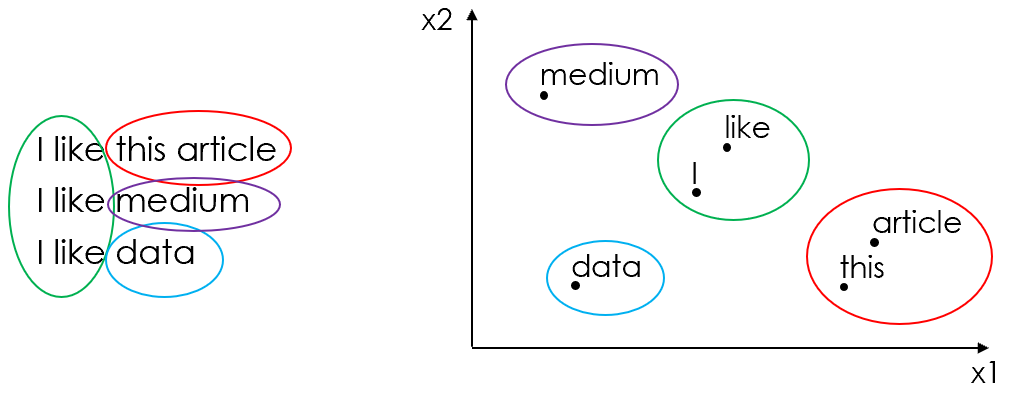
\includegraphics[width=\linewidth]{resources/pictures/tfidf-vs-embeddings.png}  % Add a visual comparison
    \end{columns}
    \textbf{Solution: Word embeddings}\newline
    Embeddings create \textbf{dense}, low-dimensional representations that retain meaning and context.
\end{frame}

\begin{frame}{What are embeddings?}
    \begin{itemize}
        \item Map words or documents into \textbf{continuous vector spaces}.
        \item Words with similar meanings have \textbf{similar vectors}.
        \item \textbf{Learned} from large text corpora using machine learning models.
    \end{itemize}
    \pause
    \textbf{Popular Examples:} Word2Vec, GloVe, fastText, BERT embeddings.
    \newline
    \begin{center}
        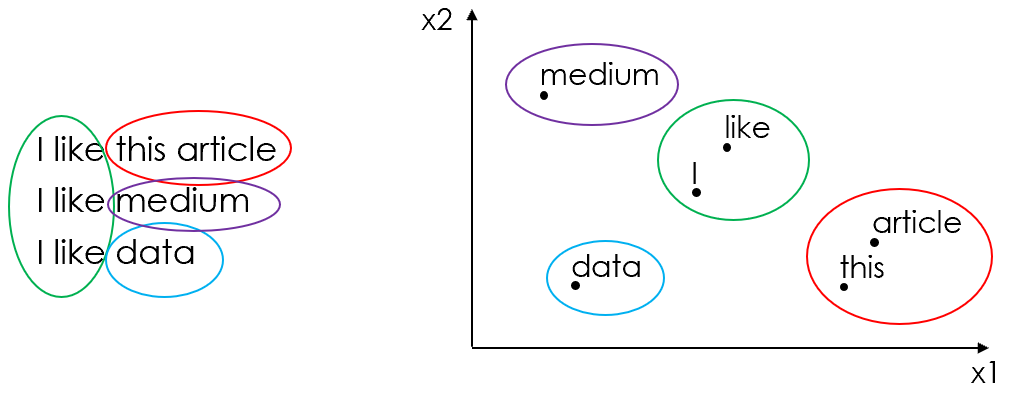
\includegraphics[width=0.8\linewidth]{resources/pictures/tfidf-vs-embeddings.png}  % Example word embedding space visualization
    \end{center}
\end{frame}

\subsection{Word embeddings}

\begin{frame}{Understanding embeddings}
	\begin{block}{What are word embeddings?}
		\begin{itemize}[<+>]
			\item No technical details here, just the general idea
			\item Word embeddings help capture the meaning of text
			\item Word embeddings are low-dimensional vector representations that capture semantic meaning
			\item Used to be state-of-the-art in NLP (but now: contextualized embeddings, e.g., BERT or GPT)
			\item \emph{``...a word is characterized by the company it keeps...''} (Firth, 1957)
		\end{itemize}
	\end{block}
\end{frame}

\begin{frame}{}
	\makebox[\linewidth]{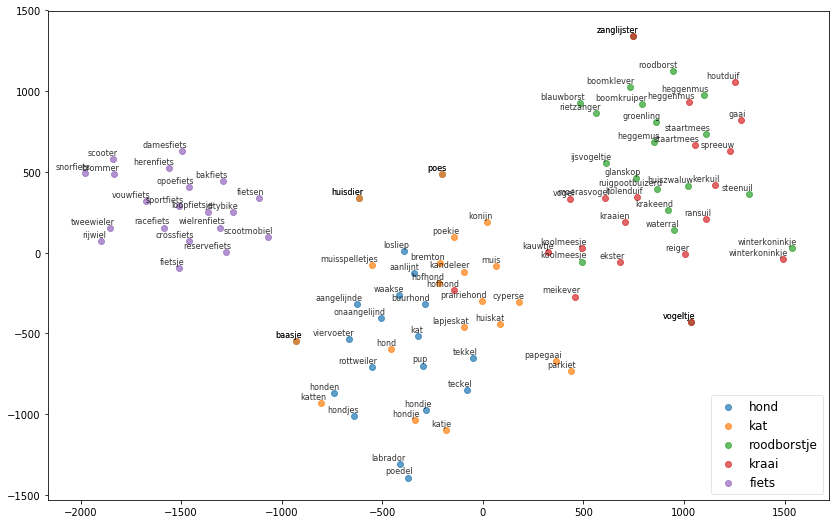
\includegraphics[width=\linewidth,height=\textheight, keepaspectratio]{resources/pictures/w2v_300_illustration.png}}
\end{frame}


\begin{frame}{}
	\makebox[\linewidth]{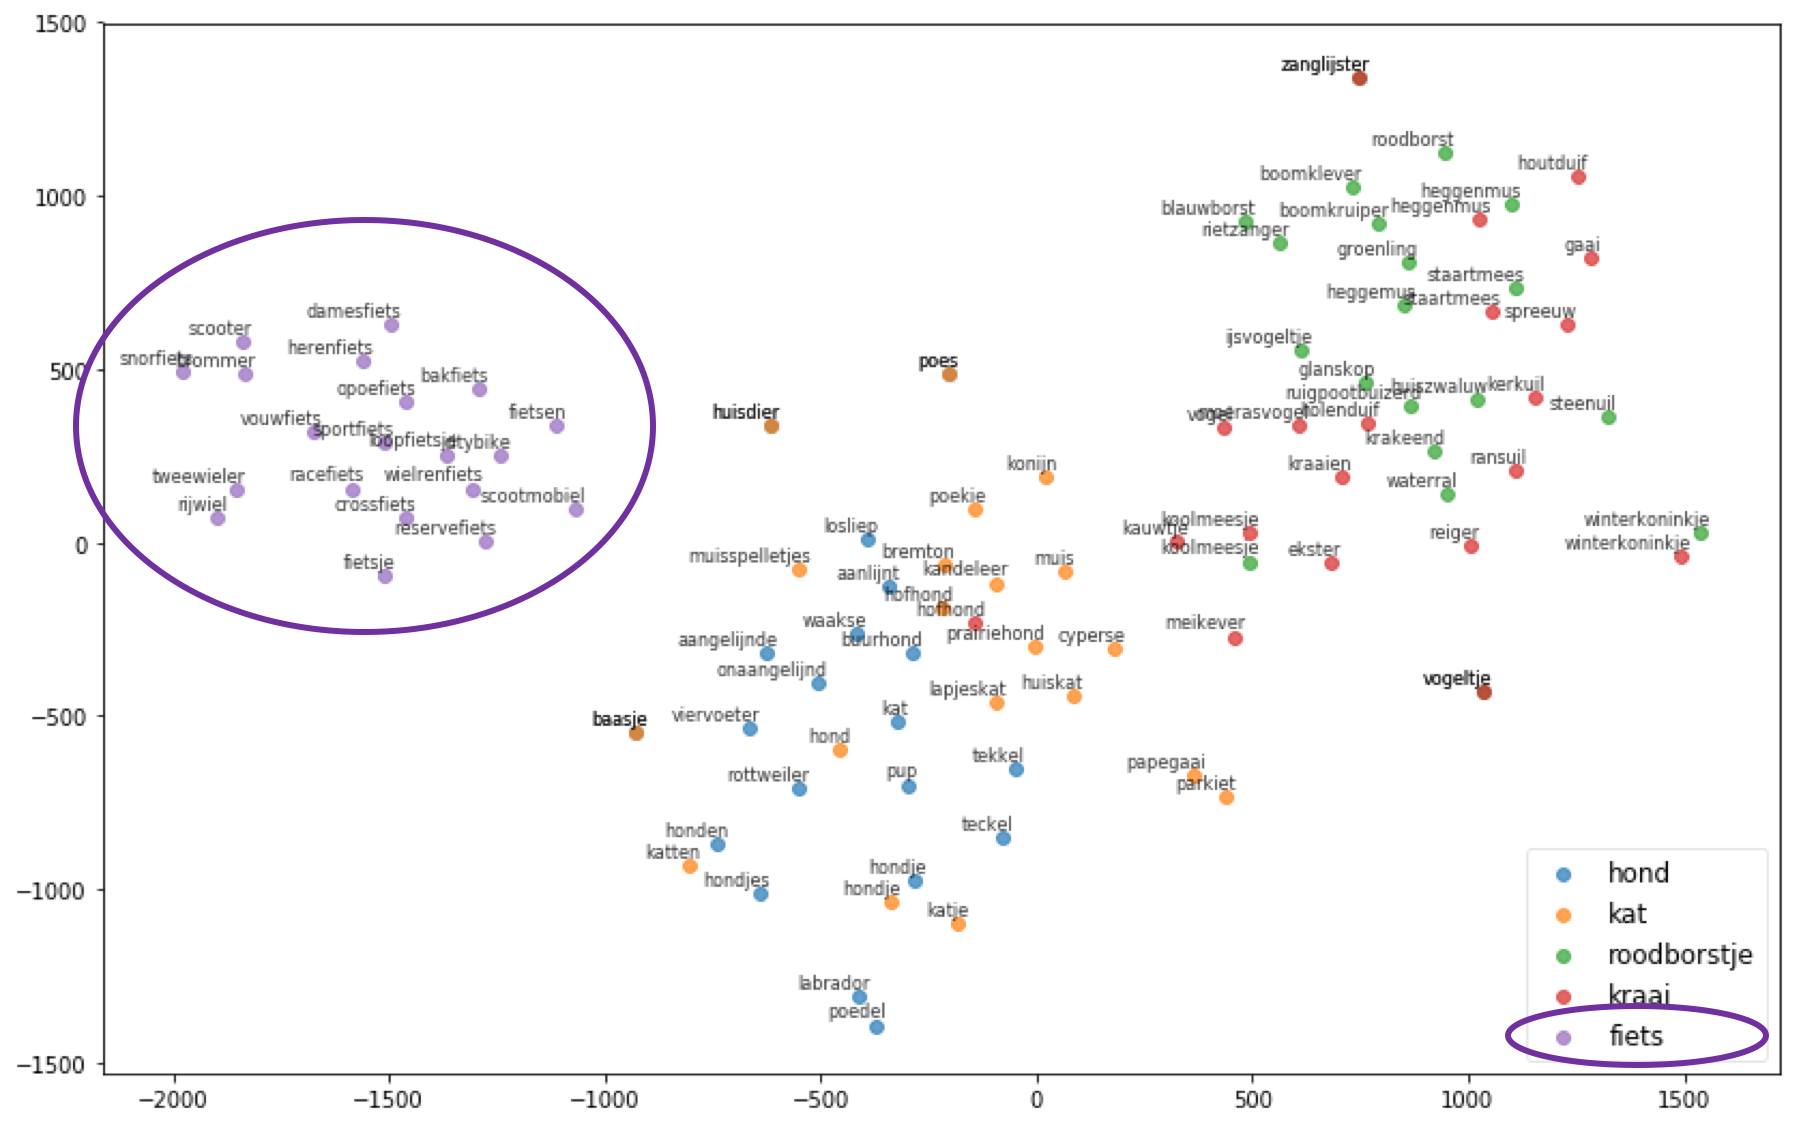
\includegraphics[width=\linewidth,height=\textheight, keepaspectratio]{resources/pictures/visual2.png}}
\end{frame}

%as can be seen, words most similar to fiets are on the left. 

\begin{frame}{}
	\makebox[\linewidth]{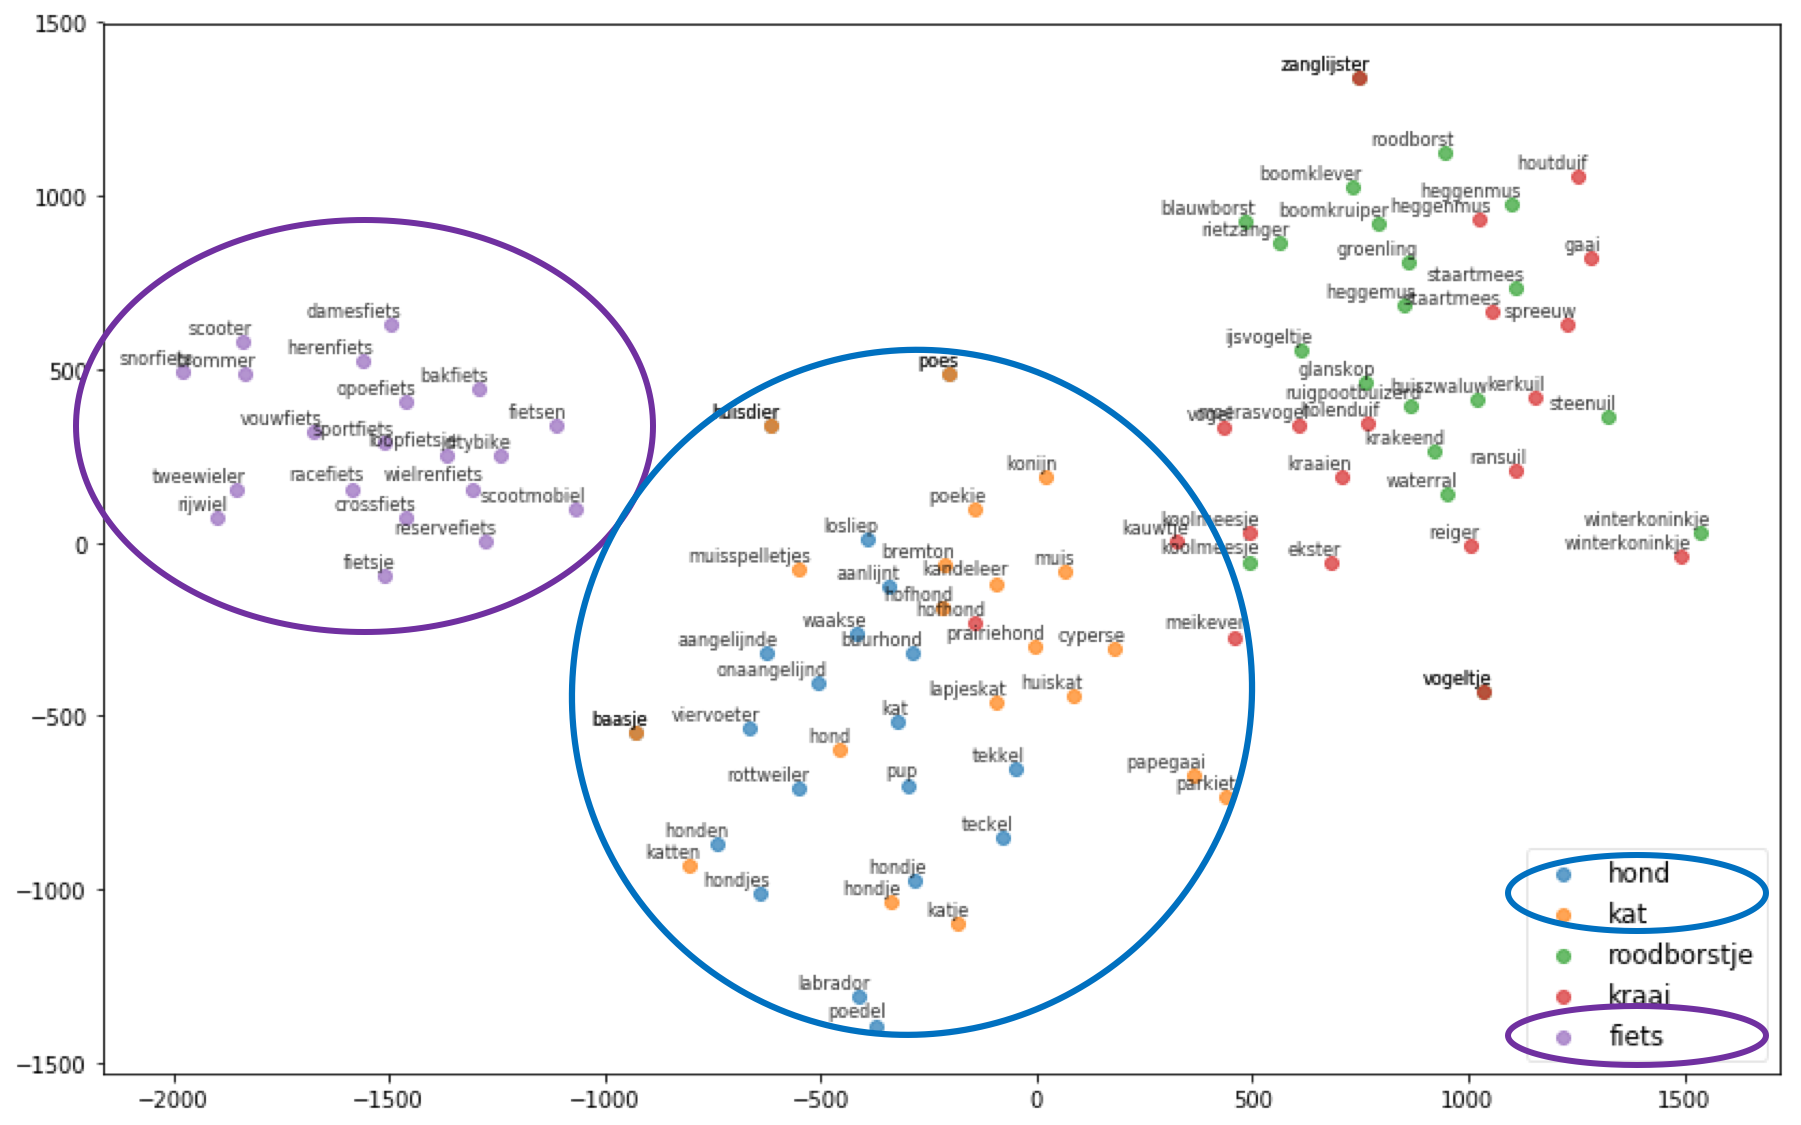
\includegraphics[width=\linewidth,height=\textheight, keepaspectratio]{resources/pictures/visual1.png}}
\end{frame}

%the model recognizes that fiets is something else from honden and katten. Both mammals and pets, dogs and cats are quite similar and appear in the same cluster.  

\begin{frame}{}
	\makebox[\linewidth]{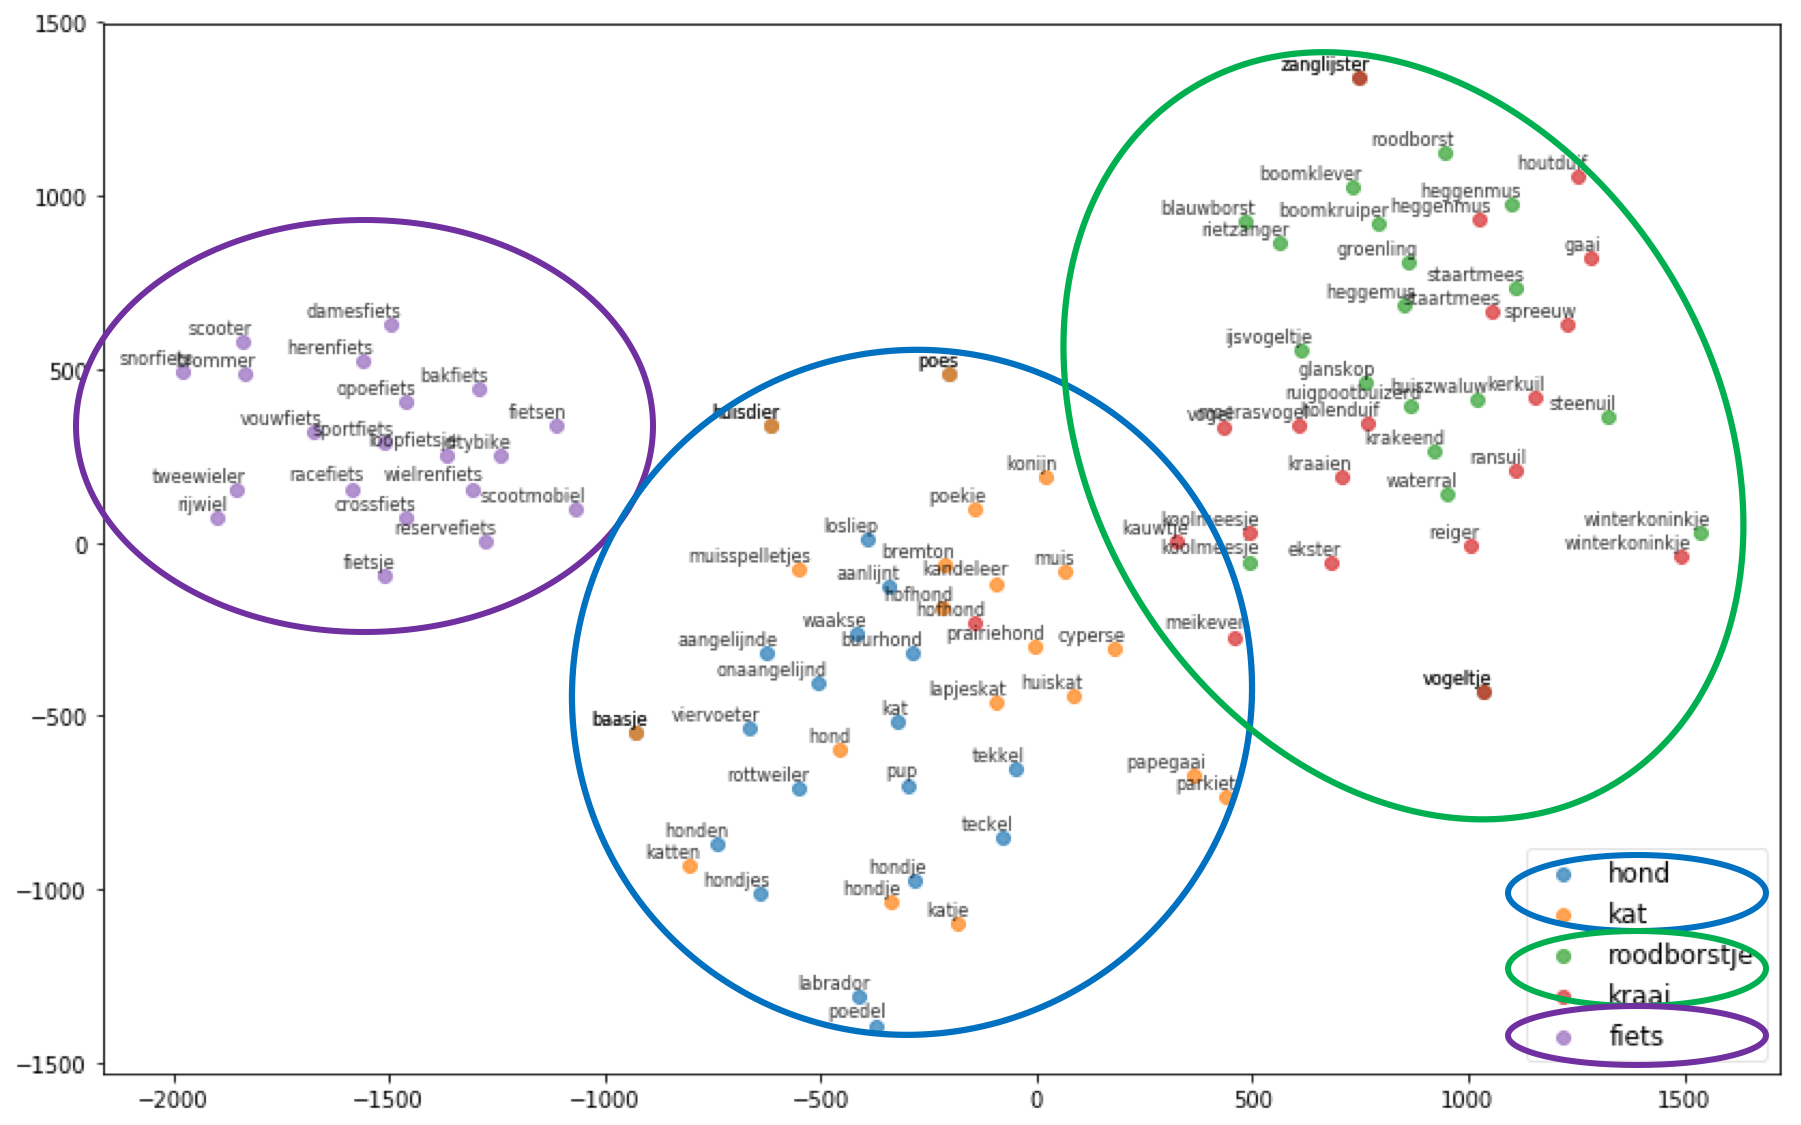
\includegraphics[width=\linewidth,height=\textheight, keepaspectratio]{resources/pictures/visual.png}}

\begin{itemize}
    \item Explore word embeddings interactively using the TensorFlow Projector.
    \item \href{https://projector.tensorflow.org/}{Click here to access the TensorFlow Projector.}
\end{itemize}

\end{frame}


\begin{frame}{How embeddings work}
    \begin{itemize}
        \item Each word (or document) is represented by a \textbf{vector} in a high-dimensional space.
        \item The model learns these vectors by predicting word co-occurrences in text.
        \item Example: \textbf{Word2Vec} uses a neural network to predict surrounding words.
    \end{itemize}
\end{frame}

\begin{frame}{Example: Word similarity with embeddings}
    \begin{columns}
        \column{0.5\textwidth}
        \textbf{Word2Vec analogy:}
        \begin{itemize}
            \item \texttt{vec("king") - vec("man") + vec("woman") = vec("queen")}
            \item Captures \textbf{semantic relationships} automatically.
            \item Unlike TF-IDF, embeddings \textbf{understand meaning}.
        \end{itemize}
        \column{0.5\textwidth}
        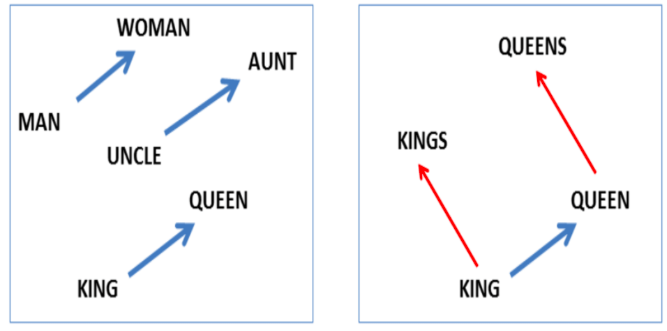
\includegraphics[width=\linewidth]{resources/pictures/embeddings.png}  % Visual representation of vector math
    \end{columns}
\end{frame}


\begin{frame}[fragile]{Example: Getting word embeddings with spaCy}
\href{https://github.com/uva-cw-ccs2/2425s2/blob/main/week02/exercise-lecture/visualize-embeddings.ipynb}{Try it out yourself.. Visualize your embeddings}
    \begin{center}
        
\includegraphics[width=0.8\linewidth]{resources/pictures/vectors.png}  
    \end{center}
\end{frame}

\begin{frame}[fragile]{Embeddings in communication science}
    \textbf{Applications:}
    \begin{itemize}
        \item \textbf{Sentiment analysis:} Understanding audience reactions on social media (\cite{rudkowsky2018more})
        \item \textbf{Topic modeling}: cross lingual topics (\cite{han2020reproducible)}
        \item \textbf{Recommender Systems:} Suggesting content based on user preferences (\cite{Loecherbach2020})
    \item \textbf{Text similarity:} Measuring the similarity between texts.
        \begin{itemize}
            \item Example: \cite{Brinberg2021}
        \end{itemize}
\end{itemize}
\textbf{Note:} We will discuss this next week.
\end{frame}


\begin{frame}{Using pretrained embeddings}
    \textbf{Why use pretrained models?}
    \begin{itemize}
        \item Trained on massive datasets (Google News, Wikipedia, etc.).
        \item Capture \textbf{rich linguistic structures}.
        \item Reduce training time and improve performance.
    \end{itemize}
    \pause
    \textbf{Popular Choices:}
    \begin{columns}
        \column{0.5\textwidth}
        \begin{itemize}
            \item Word2Vec (Google News)
            \item GloVe (Common Crawl, Wikipedia)
        \end{itemize}
        \column{0.5\textwidth}
        \begin{itemize}
            \item BERT (contextualized embeddings)
            \item fastText (subword information)
        \end{itemize}
    \end{columns}
\end{frame}

\begin{frame}[fragile]{Why Use Embeddings?}
    \begin{itemize}
        \item Capture \textbf{semantic meaning} of words.
        \item Handle \textbf{synonyms} and \textbf{related words} effectively.
        \item Work well in NLP applications: \textbf{text classification, clustering, sentiment analysis}.
        \item Used in communication science for \textbf{media analysis, misinformation detection, and social network studies}.
    \end{itemize}
\end{frame}

\begin{frame}{Key takeaways}
    \begin{itemize}
        \item Traditional methods (TF-IDF) are \textbf{limited in capturing meaning}.
        \item Word embeddings create \textbf{dense vectors} that capture relationships.
        \item Pretrained models like \textbf{Word2Vec, GloVe, and BERT} help analyze text effectively.
        \item Embeddings are \textbf{widely used} in NLP and communication science.
    \end{itemize}
\end{frame}

\end{document}

